% Options for packages loaded elsewhere
\PassOptionsToPackage{unicode}{hyperref}
\PassOptionsToPackage{hyphens}{url}
\PassOptionsToPackage{dvipsnames,svgnames,x11names}{xcolor}
%
\documentclass[
  letterpaper,
  DIV=11,
  numbers=noendperiod]{scrartcl}

\usepackage{amsmath,amssymb}
\usepackage{iftex}
\ifPDFTeX
  \usepackage[T1]{fontenc}
  \usepackage[utf8]{inputenc}
  \usepackage{textcomp} % provide euro and other symbols
\else % if luatex or xetex
  \usepackage{unicode-math}
  \defaultfontfeatures{Scale=MatchLowercase}
  \defaultfontfeatures[\rmfamily]{Ligatures=TeX,Scale=1}
\fi
\usepackage{lmodern}
\ifPDFTeX\else  
    % xetex/luatex font selection
\fi
% Use upquote if available, for straight quotes in verbatim environments
\IfFileExists{upquote.sty}{\usepackage{upquote}}{}
\IfFileExists{microtype.sty}{% use microtype if available
  \usepackage[]{microtype}
  \UseMicrotypeSet[protrusion]{basicmath} % disable protrusion for tt fonts
}{}
\makeatletter
\@ifundefined{KOMAClassName}{% if non-KOMA class
  \IfFileExists{parskip.sty}{%
    \usepackage{parskip}
  }{% else
    \setlength{\parindent}{0pt}
    \setlength{\parskip}{6pt plus 2pt minus 1pt}}
}{% if KOMA class
  \KOMAoptions{parskip=half}}
\makeatother
\usepackage{xcolor}
\setlength{\emergencystretch}{3em} % prevent overfull lines
\setcounter{secnumdepth}{-\maxdimen} % remove section numbering
% Make \paragraph and \subparagraph free-standing
\makeatletter
\ifx\paragraph\undefined\else
  \let\oldparagraph\paragraph
  \renewcommand{\paragraph}{
    \@ifstar
      \xxxParagraphStar
      \xxxParagraphNoStar
  }
  \newcommand{\xxxParagraphStar}[1]{\oldparagraph*{#1}\mbox{}}
  \newcommand{\xxxParagraphNoStar}[1]{\oldparagraph{#1}\mbox{}}
\fi
\ifx\subparagraph\undefined\else
  \let\oldsubparagraph\subparagraph
  \renewcommand{\subparagraph}{
    \@ifstar
      \xxxSubParagraphStar
      \xxxSubParagraphNoStar
  }
  \newcommand{\xxxSubParagraphStar}[1]{\oldsubparagraph*{#1}\mbox{}}
  \newcommand{\xxxSubParagraphNoStar}[1]{\oldsubparagraph{#1}\mbox{}}
\fi
\makeatother

\usepackage{color}
\usepackage{fancyvrb}
\newcommand{\VerbBar}{|}
\newcommand{\VERB}{\Verb[commandchars=\\\{\}]}
\DefineVerbatimEnvironment{Highlighting}{Verbatim}{commandchars=\\\{\}}
% Add ',fontsize=\small' for more characters per line
\usepackage{framed}
\definecolor{shadecolor}{RGB}{241,243,245}
\newenvironment{Shaded}{\begin{snugshade}}{\end{snugshade}}
\newcommand{\AlertTok}[1]{\textcolor[rgb]{0.68,0.00,0.00}{#1}}
\newcommand{\AnnotationTok}[1]{\textcolor[rgb]{0.37,0.37,0.37}{#1}}
\newcommand{\AttributeTok}[1]{\textcolor[rgb]{0.40,0.45,0.13}{#1}}
\newcommand{\BaseNTok}[1]{\textcolor[rgb]{0.68,0.00,0.00}{#1}}
\newcommand{\BuiltInTok}[1]{\textcolor[rgb]{0.00,0.23,0.31}{#1}}
\newcommand{\CharTok}[1]{\textcolor[rgb]{0.13,0.47,0.30}{#1}}
\newcommand{\CommentTok}[1]{\textcolor[rgb]{0.37,0.37,0.37}{#1}}
\newcommand{\CommentVarTok}[1]{\textcolor[rgb]{0.37,0.37,0.37}{\textit{#1}}}
\newcommand{\ConstantTok}[1]{\textcolor[rgb]{0.56,0.35,0.01}{#1}}
\newcommand{\ControlFlowTok}[1]{\textcolor[rgb]{0.00,0.23,0.31}{\textbf{#1}}}
\newcommand{\DataTypeTok}[1]{\textcolor[rgb]{0.68,0.00,0.00}{#1}}
\newcommand{\DecValTok}[1]{\textcolor[rgb]{0.68,0.00,0.00}{#1}}
\newcommand{\DocumentationTok}[1]{\textcolor[rgb]{0.37,0.37,0.37}{\textit{#1}}}
\newcommand{\ErrorTok}[1]{\textcolor[rgb]{0.68,0.00,0.00}{#1}}
\newcommand{\ExtensionTok}[1]{\textcolor[rgb]{0.00,0.23,0.31}{#1}}
\newcommand{\FloatTok}[1]{\textcolor[rgb]{0.68,0.00,0.00}{#1}}
\newcommand{\FunctionTok}[1]{\textcolor[rgb]{0.28,0.35,0.67}{#1}}
\newcommand{\ImportTok}[1]{\textcolor[rgb]{0.00,0.46,0.62}{#1}}
\newcommand{\InformationTok}[1]{\textcolor[rgb]{0.37,0.37,0.37}{#1}}
\newcommand{\KeywordTok}[1]{\textcolor[rgb]{0.00,0.23,0.31}{\textbf{#1}}}
\newcommand{\NormalTok}[1]{\textcolor[rgb]{0.00,0.23,0.31}{#1}}
\newcommand{\OperatorTok}[1]{\textcolor[rgb]{0.37,0.37,0.37}{#1}}
\newcommand{\OtherTok}[1]{\textcolor[rgb]{0.00,0.23,0.31}{#1}}
\newcommand{\PreprocessorTok}[1]{\textcolor[rgb]{0.68,0.00,0.00}{#1}}
\newcommand{\RegionMarkerTok}[1]{\textcolor[rgb]{0.00,0.23,0.31}{#1}}
\newcommand{\SpecialCharTok}[1]{\textcolor[rgb]{0.37,0.37,0.37}{#1}}
\newcommand{\SpecialStringTok}[1]{\textcolor[rgb]{0.13,0.47,0.30}{#1}}
\newcommand{\StringTok}[1]{\textcolor[rgb]{0.13,0.47,0.30}{#1}}
\newcommand{\VariableTok}[1]{\textcolor[rgb]{0.07,0.07,0.07}{#1}}
\newcommand{\VerbatimStringTok}[1]{\textcolor[rgb]{0.13,0.47,0.30}{#1}}
\newcommand{\WarningTok}[1]{\textcolor[rgb]{0.37,0.37,0.37}{\textit{#1}}}

\providecommand{\tightlist}{%
  \setlength{\itemsep}{0pt}\setlength{\parskip}{0pt}}\usepackage{longtable,booktabs,array}
\usepackage{calc} % for calculating minipage widths
% Correct order of tables after \paragraph or \subparagraph
\usepackage{etoolbox}
\makeatletter
\patchcmd\longtable{\par}{\if@noskipsec\mbox{}\fi\par}{}{}
\makeatother
% Allow footnotes in longtable head/foot
\IfFileExists{footnotehyper.sty}{\usepackage{footnotehyper}}{\usepackage{footnote}}
\makesavenoteenv{longtable}
\usepackage{graphicx}
\makeatletter
\def\maxwidth{\ifdim\Gin@nat@width>\linewidth\linewidth\else\Gin@nat@width\fi}
\def\maxheight{\ifdim\Gin@nat@height>\textheight\textheight\else\Gin@nat@height\fi}
\makeatother
% Scale images if necessary, so that they will not overflow the page
% margins by default, and it is still possible to overwrite the defaults
% using explicit options in \includegraphics[width, height, ...]{}
\setkeys{Gin}{width=\maxwidth,height=\maxheight,keepaspectratio}
% Set default figure placement to htbp
\makeatletter
\def\fps@figure{htbp}
\makeatother

\KOMAoption{captions}{tableheading}
\makeatletter
\@ifpackageloaded{caption}{}{\usepackage{caption}}
\AtBeginDocument{%
\ifdefined\contentsname
  \renewcommand*\contentsname{Table of contents}
\else
  \newcommand\contentsname{Table of contents}
\fi
\ifdefined\listfigurename
  \renewcommand*\listfigurename{List of Figures}
\else
  \newcommand\listfigurename{List of Figures}
\fi
\ifdefined\listtablename
  \renewcommand*\listtablename{List of Tables}
\else
  \newcommand\listtablename{List of Tables}
\fi
\ifdefined\figurename
  \renewcommand*\figurename{Figure}
\else
  \newcommand\figurename{Figure}
\fi
\ifdefined\tablename
  \renewcommand*\tablename{Table}
\else
  \newcommand\tablename{Table}
\fi
}
\@ifpackageloaded{float}{}{\usepackage{float}}
\floatstyle{ruled}
\@ifundefined{c@chapter}{\newfloat{codelisting}{h}{lop}}{\newfloat{codelisting}{h}{lop}[chapter]}
\floatname{codelisting}{Listing}
\newcommand*\listoflistings{\listof{codelisting}{List of Listings}}
\makeatother
\makeatletter
\makeatother
\makeatletter
\@ifpackageloaded{caption}{}{\usepackage{caption}}
\@ifpackageloaded{subcaption}{}{\usepackage{subcaption}}
\makeatother

\ifLuaTeX
  \usepackage{selnolig}  % disable illegal ligatures
\fi
\usepackage{bookmark}

\IfFileExists{xurl.sty}{\usepackage{xurl}}{} % add URL line breaks if available
\urlstyle{same} % disable monospaced font for URLs
\hypersetup{
  pdftitle={Take-home Exercise 1},
  pdfauthor={Marga Thura},
  colorlinks=true,
  linkcolor={blue},
  filecolor={Maroon},
  citecolor={Blue},
  urlcolor={Blue},
  pdfcreator={LaTeX via pandoc}}


\title{Take-home Exercise 1}
\author{Marga Thura}
\date{2025-05-02}

\begin{document}
\maketitle


\section{\texorpdfstring{\textbf{Visualizing the Age and Gender
Landscape of
Singapore}}{Visualizing the Age and Gender Landscape of Singapore}}\label{visualizing-the-age-and-gender-landscape-of-singapore}

\section{1 Overview}\label{overview}

\subsection{1.1 Setting the scene}\label{setting-the-scene}

A local online media company that publishes daily content on digital
platforms is planning to release an article on demographic structures
and distribution of Singapore in 2024. This project will explore the
demographic structure of Singapore's resident population as of June
2024, which aims to uncover both national and regional trends in age
distribution, gender composition, and population disparities across
planning areas.

\subsection{1.2 Tasks}\label{tasks}

As the graphical editor of the media company, this project aim to:

\begin{enumerate}
\def\labelenumi{\arabic{enumi}.}
\item
  Clean and preprocess the demographic dataset.
\item
  Design and generate three targeted data visualizations:
\end{enumerate}

\begin{itemize}
\item
  \textbf{Top 10 Planning Areas by Total Population}: A horizontal bar
  chart focusing on the ten most populous planning areas to highlight
  urban population concentration, particularly in areas like Tampines,
  Bedok, and Sengkang.
\item
  \textbf{Population Pyramid by Age and Sex}: A detailed pyramid chart
  that illustrates Singapore's national age and gender structure,
  revealing the dominance of the working-age population, the presence of
  an aging society, and gender differences in older age groups.
\end{itemize}

\begin{itemize}
\tightlist
\item
  \textbf{Age and Gender Distribution in Top 5 Planning Areas}: A set of
  stacked bar and ridgeline plots showing how population varies by age
  group and gender within the top five planning areas, offering insights
  into regional differences in youth, working-age, and elderly
  populations.
\end{itemize}

\begin{enumerate}
\def\labelenumi{\arabic{enumi}.}
\setcounter{enumi}{2}
\tightlist
\item
  Summarize key insights for each visualization to support the
  narrative.
\end{enumerate}

\section{2 The Data}\label{the-data}

The official dataset ``Singapore Residents by Planning Area / Subzone,
Single Year of Age and Sex'' retrieve from
\href{https://www.singstat.gov.sg/}{department of statistics} will be
used to explore.

\begin{Shaded}
\begin{Highlighting}[]
\CommentTok{\# Load necessary library}
\FunctionTok{library}\NormalTok{(readr)}

\CommentTok{\# Read the CSV file from the specified relative path}
\NormalTok{respopagesex2024 }\OtherTok{\textless{}{-}} \FunctionTok{read\_csv}\NormalTok{(}\StringTok{"TakeHome\_01/respopagesex2024.csv"}\NormalTok{)}
\end{Highlighting}
\end{Shaded}

\subsection{2.1 Loading Packages}\label{loading-packages}

The code chunk below uses p\_load() of pacman package to check if
tidyverse packages are installed in the computer. If they are, then they
will be launched into R.

\begin{Shaded}
\begin{Highlighting}[]
\NormalTok{pacman}\SpecialCharTok{::}\FunctionTok{p\_load}\NormalTok{(tidyverse)}
\end{Highlighting}
\end{Shaded}

Beside tidyverse, following R packages will be used:

\begin{itemize}
\item
  \textbf{ggrepel:} an R package provides geoms for ggplot2 to repel
  overlapping text labels.
\item
  \textbf{ggthemes:} an R package provides some extra themes, geoms, and
  scales for `ggplot2'.
\item
  \textbf{hrbrthemes:} an R package provides typography-centric themes
  and theme components for ggplot2.
\item
  \textbf{patchwork:} an R package for preparing composite figure
  created using ggplot2.
\item
  \textbf{haven:} Enables reading and writing of data files from
  statistical software packages like SPSS, Stata, and SAS.
\item
  \textbf{ggiraph:} for making `ggplot' graphics interactive.
\item
  \textbf{plotly}: R library for plotting interactive statistical
  graphs.
\item
  \textbf{DT:} provides an R interface to the JavaScript library
  DataTables that create interactive table on html page.
\item
  \textbf{knitr:} Facilitates dynamic report generation by integrating R
  code into documents (used in R Markdown).
\item
  \textbf{scales:} Provides functions for scaling axes and legends in
  ggplot2 plots, including formatting numbers and dates.
\item
  \textbf{ggridges:} Allows creation of ridgeline plots (overlapping
  density plots) in ggplot2.
\item
  \textbf{ggpubr:} Enhances ggplot2 with publication-ready themes and
  functions for common tasks like adding statistical comparisons.
\item
  \textbf{gganimate:} Adds animation capabilities to ggplot2
  visualizations.
\item
  \textbf{gapminder:} An excerpt of the data available at Gapminder.org.
\item
  \textbf{ggdist:} Supports visualizations of distributions and
  uncertainty (e.g., intervals, densities) in ggplot2.
\item
  \textbf{ggtext:} Enables advanced text rendering (e.g., HTML/Markdown)
  in ggplot2 titles, subtitles, and labels
\item
  \textbf{ggalt:} Provides alternative geoms and statistical
  transformations not available in core ggplot2.
\item
  \textbf{cowplot:} Offers streamlined tools to align and arrange
  ggplot2-based plots into panels.
\end{itemize}

\begin{Shaded}
\begin{Highlighting}[]
\NormalTok{pacman}\SpecialCharTok{::}\FunctionTok{p\_load}\NormalTok{(tidyverse, ggrepel, ggthemes, }
\NormalTok{               hrbrthemes, patchwork, }
\NormalTok{               haven, ggiraph, plotly, DT, }
\NormalTok{               knitr, scales,}
\NormalTok{               ggridges, ggpubr, }
\NormalTok{               gganimate, gapminder, ggdist, }
\NormalTok{               ggtext, ggalt,}
\NormalTok{               cowplot)}
\end{Highlighting}
\end{Shaded}

\subsection{2.2 Cleaning data}\label{cleaning-data}

To prepare the dataset for all tasks, the following code will loads,
cleans, and prepares the demographic data (respopagesex2024.csv) for
analysis and visualization to make sure:

\begin{itemize}
\item
  All numeric columns are actually numeric (for calculations)
\item
  Categorical columns behave predictably (for grouping)
\item
  Only analyzing valid population entries (no missing or zero values).
\end{itemize}

\begin{Shaded}
\begin{Highlighting}[]
\FunctionTok{library}\NormalTok{(readr)}
\FunctionTok{library}\NormalTok{(dplyr)}

\CommentTok{\# Load the dataset}
\NormalTok{respop }\OtherTok{\textless{}{-}} \FunctionTok{read\_csv}\NormalTok{(}\StringTok{"TakeHome\_01/respopagesex2024.csv"}\NormalTok{)}

\CommentTok{\# Convert types and clean}
\NormalTok{respop\_clean }\OtherTok{\textless{}{-}}\NormalTok{ respop }\SpecialCharTok{\%\textgreater{}\%}
  \FunctionTok{mutate}\NormalTok{(}
    \AttributeTok{Pop =} \FunctionTok{as.numeric}\NormalTok{(Pop),}
    \AttributeTok{Age =} \FunctionTok{as.numeric}\NormalTok{(Age),}
    \AttributeTok{PA =} \FunctionTok{as.factor}\NormalTok{(PA),}
    \AttributeTok{SZ =} \FunctionTok{as.factor}\NormalTok{(SZ),}
    \AttributeTok{Sex =} \FunctionTok{factor}\NormalTok{(Sex, }\AttributeTok{levels =} \FunctionTok{c}\NormalTok{(}\StringTok{"Males"}\NormalTok{, }\StringTok{"Females"}\NormalTok{))}
\NormalTok{  ) }\SpecialCharTok{\%\textgreater{}\%}
  \FunctionTok{filter}\NormalTok{(}\SpecialCharTok{!}\FunctionTok{is.na}\NormalTok{(Pop), Pop }\SpecialCharTok{\textgreater{}} \DecValTok{0}\NormalTok{)}
\end{Highlighting}
\end{Shaded}

The following code chunk will loads the dataset.

\begin{itemize}
\item
  Cleans it by ensuring population values are numeric and valid.
\item
  Aggregates population totals by planning area.
\item
  Outputs a basic statistical overview of how population is distributed
  across Singapore's planning areas.
\end{itemize}

\begin{Shaded}
\begin{Highlighting}[]
  \FunctionTok{library}\NormalTok{(readr)}
  \FunctionTok{library}\NormalTok{(dplyr)}
  \FunctionTok{library}\NormalTok{(ggplot2)}
  \FunctionTok{library}\NormalTok{(scales)}

  \CommentTok{\# Load and summarize population data}
\NormalTok{  respopagesex2024 }\OtherTok{\textless{}{-}} \FunctionTok{read\_csv}\NormalTok{(}\StringTok{"TakeHome\_01/respopagesex2024.csv"}\NormalTok{)}
\NormalTok{  pop\_by\_pa }\OtherTok{\textless{}{-}}\NormalTok{ respopagesex2024 }\SpecialCharTok{\%\textgreater{}\%}
    \FunctionTok{mutate}\NormalTok{(}\AttributeTok{Pop =} \FunctionTok{as.numeric}\NormalTok{(Pop)) }\SpecialCharTok{\%\textgreater{}\%}
    \FunctionTok{filter}\NormalTok{(}\SpecialCharTok{!}\FunctionTok{is.na}\NormalTok{(Pop) }\SpecialCharTok{\&}\NormalTok{ Pop }\SpecialCharTok{\textgreater{}} \DecValTok{0}\NormalTok{) }\SpecialCharTok{\%\textgreater{}\%}
    \FunctionTok{group\_by}\NormalTok{(PA) }\SpecialCharTok{\%\textgreater{}\%}
    \FunctionTok{summarise}\NormalTok{(}\AttributeTok{Total\_Pop =} \FunctionTok{sum}\NormalTok{(Pop, }\AttributeTok{na.rm =} \ConstantTok{TRUE}\NormalTok{))}

  \CommentTok{\# Check population range}
  \FunctionTok{print}\NormalTok{(}\FunctionTok{summary}\NormalTok{(pop\_by\_pa}\SpecialCharTok{$}\NormalTok{Total\_Pop))}
\end{Highlighting}
\end{Shaded}

\begin{verbatim}
   Min. 1st Qu.  Median    Mean 3rd Qu.    Max. 
    140    8432   94700   99846  157685  284950 
\end{verbatim}

The following code chunk will loads the dataset, deep clean and check
for missing or abnormal entries.

\begin{Shaded}
\begin{Highlighting}[]
\FunctionTok{summary}\NormalTok{(respopagesex2024)}
\end{Highlighting}
\end{Shaded}

\begin{verbatim}
      PA                 SZ                Age                Sex           
 Length:60424       Length:60424       Length:60424       Length:60424      
 Class :character   Class :character   Class :character   Class :character  
 Mode  :character   Mode  :character   Mode  :character   Mode  :character  
                                                                            
                                                                            
                                                                            
      Pop              Time     
 Min.   :   0.0   Min.   :2024  
 1st Qu.:   0.0   1st Qu.:2024  
 Median :  20.0   Median :2024  
 Mean   :  69.4   Mean   :2024  
 3rd Qu.:  90.0   3rd Qu.:2024  
 Max.   :1180.0   Max.   :2024  
\end{verbatim}

\begin{Shaded}
\begin{Highlighting}[]
\FunctionTok{any}\NormalTok{(}\FunctionTok{is.na}\NormalTok{(respopagesex2024}\SpecialCharTok{$}\NormalTok{PA))}
\end{Highlighting}
\end{Shaded}

\begin{verbatim}
[1] FALSE
\end{verbatim}

\begin{Shaded}
\begin{Highlighting}[]
\FunctionTok{any}\NormalTok{(}\FunctionTok{is.na}\NormalTok{(respopagesex2024}\SpecialCharTok{$}\NormalTok{SZ))}
\end{Highlighting}
\end{Shaded}

\begin{verbatim}
[1] FALSE
\end{verbatim}

\begin{Shaded}
\begin{Highlighting}[]
\FunctionTok{any}\NormalTok{(respopagesex2024}\SpecialCharTok{$}\NormalTok{PA }\SpecialCharTok{==} \StringTok{""}\NormalTok{)}
\end{Highlighting}
\end{Shaded}

\begin{verbatim}
[1] FALSE
\end{verbatim}

\section{3 Distribution of Population Across Singapore's Planning
Areas}\label{distribution-of-population-across-singapores-planning-areas}

\subsection{Plot 1}\label{plot-1}

\begin{Shaded}
\begin{Highlighting}[]
\FunctionTok{library}\NormalTok{(dplyr)}
\FunctionTok{library}\NormalTok{(ggplot2)}
\FunctionTok{library}\NormalTok{(scales)}
\FunctionTok{library}\NormalTok{(readr)}

\CommentTok{\# Load data}
\NormalTok{respopagesex2024 }\OtherTok{\textless{}{-}} \FunctionTok{read\_csv}\NormalTok{(}\StringTok{"TakeHome\_01/respopagesex2024.csv"}\NormalTok{)}

\CommentTok{\# Clean and summarize population by PA}
\NormalTok{pop\_by\_pa }\OtherTok{\textless{}{-}}\NormalTok{ respopagesex2024 }\SpecialCharTok{\%\textgreater{}\%}
  \FunctionTok{mutate}\NormalTok{(}\AttributeTok{Pop =} \FunctionTok{as.numeric}\NormalTok{(Pop)) }\SpecialCharTok{\%\textgreater{}\%}
  \FunctionTok{filter}\NormalTok{(}\SpecialCharTok{!}\FunctionTok{is.na}\NormalTok{(Pop) }\SpecialCharTok{\&}\NormalTok{ Pop }\SpecialCharTok{\textgreater{}} \DecValTok{0}\NormalTok{) }\SpecialCharTok{\%\textgreater{}\%}
  \FunctionTok{group\_by}\NormalTok{(PA) }\SpecialCharTok{\%\textgreater{}\%}
  \FunctionTok{summarise}\NormalTok{(}
    \AttributeTok{Total\_Pop =} \FunctionTok{sum}\NormalTok{(Pop, }\AttributeTok{na.rm =} \ConstantTok{TRUE}\NormalTok{),}
    \AttributeTok{Num\_Subzones =} \FunctionTok{n\_distinct}\NormalTok{(SZ)}
\NormalTok{  ) }\SpecialCharTok{\%\textgreater{}\%}
  \FunctionTok{arrange}\NormalTok{(}\FunctionTok{desc}\NormalTok{(Total\_Pop)) }\SpecialCharTok{\%\textgreater{}\%}
  \FunctionTok{slice\_max}\NormalTok{(}\AttributeTok{order\_by =}\NormalTok{ Total\_Pop, }\AttributeTok{n =} \DecValTok{10}\NormalTok{) }

\CommentTok{\# Plot}
\FunctionTok{ggplot}\NormalTok{(pop\_by\_pa, }\FunctionTok{aes}\NormalTok{(}\AttributeTok{x =} \FunctionTok{reorder}\NormalTok{(PA, Total\_Pop), }\AttributeTok{y =}\NormalTok{ Total\_Pop)) }\SpecialCharTok{+}
  \FunctionTok{geom\_bar}\NormalTok{(}\AttributeTok{stat =} \StringTok{"identity"}\NormalTok{, }\AttributeTok{fill =} \StringTok{"grey70"}\NormalTok{, }\AttributeTok{color =} \StringTok{"grey90"}\NormalTok{) }\SpecialCharTok{+}
  \FunctionTok{geom\_text}\NormalTok{(}\FunctionTok{aes}\NormalTok{(}\AttributeTok{label =} \FunctionTok{comma}\NormalTok{(Total\_Pop)), }\AttributeTok{hjust =} \SpecialCharTok{{-}}\FloatTok{0.1}\NormalTok{, }\AttributeTok{size =} \FloatTok{3.5}\NormalTok{) }\SpecialCharTok{+}  \CommentTok{\# Add labels}
  \FunctionTok{coord\_flip}\NormalTok{() }\SpecialCharTok{+}  \CommentTok{\# Horizontal bars}
  \FunctionTok{theme\_minimal}\NormalTok{() }\SpecialCharTok{+}
  \FunctionTok{labs}\NormalTok{(}
    \AttributeTok{title =} \StringTok{"Top 10 Most Populous Planning Areas (2024)"}\NormalTok{,}
    \AttributeTok{x =} \StringTok{"Planning Area"}\NormalTok{,}
    \AttributeTok{y =} \StringTok{"Total Population"}
\NormalTok{  ) }\SpecialCharTok{+}
  \FunctionTok{scale\_y\_continuous}\NormalTok{(}
    \AttributeTok{labels =}\NormalTok{ comma,}
    \AttributeTok{limits =} \FunctionTok{c}\NormalTok{(}\DecValTok{0}\NormalTok{, }\FunctionTok{max}\NormalTok{(pop\_by\_pa}\SpecialCharTok{$}\NormalTok{Total\_Pop) }\SpecialCharTok{*} \FloatTok{1.1}\NormalTok{)  }\CommentTok{\# Extra space for text}
\NormalTok{  )}
\end{Highlighting}
\end{Shaded}

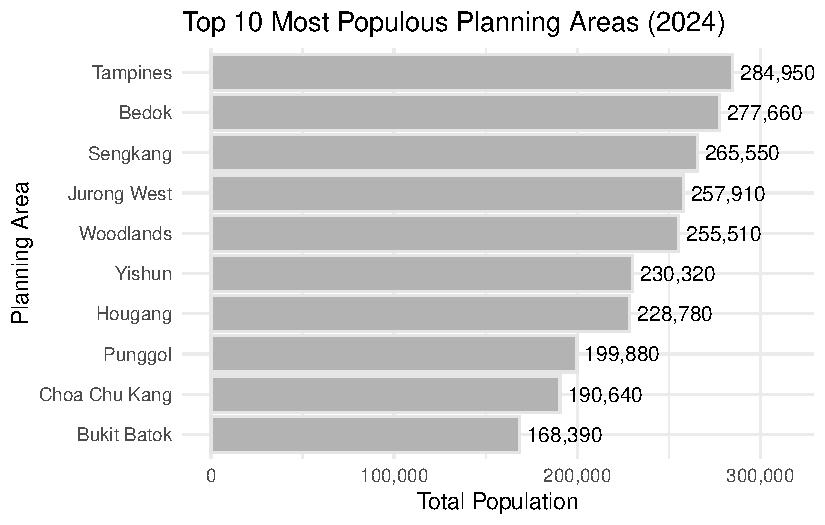
\includegraphics{Take-home_Ex01_files/figure-pdf/unnamed-chunk-7-1.pdf}

\subsection{Plot 2}\label{plot-2}

\begin{Shaded}
\begin{Highlighting}[]
\CommentTok{\# Disable scientific notation globally}
\FunctionTok{options}\NormalTok{(}\AttributeTok{scipen =} \DecValTok{999}\NormalTok{)}

\CommentTok{\# Load data}
\NormalTok{respopagesex2024 }\OtherTok{\textless{}{-}} \FunctionTok{read\_csv}\NormalTok{(}\StringTok{"TakeHome\_01/respopagesex2024.csv"}\NormalTok{)}

\CommentTok{\# Trim whitespace from PA and SZ}
\NormalTok{respopagesex2024 }\OtherTok{\textless{}{-}}\NormalTok{ respopagesex2024 }\SpecialCharTok{\%\textgreater{}\%}
  \FunctionTok{mutate}\NormalTok{(}
    \AttributeTok{PA =} \FunctionTok{trimws}\NormalTok{(PA),}
    \AttributeTok{SZ =} \FunctionTok{trimws}\NormalTok{(SZ)}
\NormalTok{  )}

\CommentTok{\# Clean and summarize population by PA, including subzone count}
\NormalTok{pop\_by\_pa }\OtherTok{\textless{}{-}}\NormalTok{ respopagesex2024 }\SpecialCharTok{\%\textgreater{}\%}
  \FunctionTok{mutate}\NormalTok{(}\AttributeTok{Pop =} \FunctionTok{as.numeric}\NormalTok{(Pop)) }\SpecialCharTok{\%\textgreater{}\%}
  \FunctionTok{filter}\NormalTok{(}\SpecialCharTok{!}\FunctionTok{is.na}\NormalTok{(Pop) }\SpecialCharTok{\&}\NormalTok{ Pop }\SpecialCharTok{\textgreater{}} \DecValTok{0}\NormalTok{) }\SpecialCharTok{\%\textgreater{}\%}
  \FunctionTok{group\_by}\NormalTok{(PA) }\SpecialCharTok{\%\textgreater{}\%}
  \FunctionTok{summarise}\NormalTok{(}
    \AttributeTok{Total\_Pop =} \FunctionTok{sum}\NormalTok{(Pop, }\AttributeTok{na.rm =} \ConstantTok{TRUE}\NormalTok{),}
    \AttributeTok{Num\_Subzones =} \FunctionTok{n\_distinct}\NormalTok{(SZ)  }\CommentTok{\# Count unique subzones per PA}
\NormalTok{  ) }\SpecialCharTok{\%\textgreater{}\%}
  \FunctionTok{arrange}\NormalTok{(}\FunctionTok{desc}\NormalTok{(Total\_Pop))}

\CommentTok{\# Create bar chart}
\NormalTok{p }\OtherTok{\textless{}{-}} \FunctionTok{ggplot}\NormalTok{(}\AttributeTok{data =}\NormalTok{ pop\_by\_pa, }\FunctionTok{aes}\NormalTok{(}\AttributeTok{x =} \FunctionTok{reorder}\NormalTok{(PA, Total\_Pop), }\AttributeTok{y =}\NormalTok{ Total\_Pop)) }\SpecialCharTok{+}
  \FunctionTok{geom\_bar}\NormalTok{(}
    \AttributeTok{stat =} \StringTok{"identity"}\NormalTok{,}
    \AttributeTok{fill =} \StringTok{"grey70"}\NormalTok{,}
    \AttributeTok{color =} \StringTok{"grey90"}
\NormalTok{  ) }\SpecialCharTok{+}
  \FunctionTok{geom\_text}\NormalTok{(}
    \FunctionTok{aes}\NormalTok{(}\AttributeTok{label =} \FunctionTok{comma}\NormalTok{(Total\_Pop)),}
    \AttributeTok{angle =} \DecValTok{90}\NormalTok{,      }\CommentTok{\# Keep text horizontal}
    \AttributeTok{hjust =} \FloatTok{0.5}\NormalTok{,    }\CommentTok{\# Center horizontally}
    \AttributeTok{vjust =} \SpecialCharTok{{-}}\FloatTok{0.5}\NormalTok{,   }\CommentTok{\# Above the bar}
    \AttributeTok{size =} \DecValTok{3}
\NormalTok{  ) }\SpecialCharTok{+}
  \FunctionTok{theme\_bw}\NormalTok{() }\SpecialCharTok{+}
  \FunctionTok{ggtitle}\NormalTok{(}\StringTok{"Population Per Planning Area (2024)"}\NormalTok{) }\SpecialCharTok{+}
  \FunctionTok{xlab}\NormalTok{(}\StringTok{"Planning Area"}\NormalTok{) }\SpecialCharTok{+}
  \FunctionTok{ylab}\NormalTok{(}\StringTok{"Total Population"}\NormalTok{) }\SpecialCharTok{+}
  \FunctionTok{theme}\NormalTok{(}
    \AttributeTok{axis.text.x =} \FunctionTok{element\_text}\NormalTok{(}\AttributeTok{angle =} \DecValTok{55}\NormalTok{, }\AttributeTok{hjust =} \DecValTok{1}\NormalTok{)}
\NormalTok{  ) }\SpecialCharTok{+}
  \FunctionTok{scale\_y\_continuous}\NormalTok{(}
    \AttributeTok{labels =}\NormalTok{ comma,}
    \AttributeTok{breaks =} \FunctionTok{seq}\NormalTok{(}\DecValTok{0}\NormalTok{, }\FunctionTok{ceiling}\NormalTok{(}\FunctionTok{max}\NormalTok{(pop\_by\_pa}\SpecialCharTok{$}\NormalTok{Total\_Pop, }\AttributeTok{na.rm =} \ConstantTok{TRUE}\NormalTok{) }\SpecialCharTok{/} \DecValTok{100000}\NormalTok{) }\SpecialCharTok{*} \DecValTok{100000}\NormalTok{, }\AttributeTok{by =} \DecValTok{100000}\NormalTok{),}
    \AttributeTok{limits =} \FunctionTok{c}\NormalTok{(}\DecValTok{0}\NormalTok{, }\FunctionTok{ceiling}\NormalTok{(}\FunctionTok{max}\NormalTok{(pop\_by\_pa}\SpecialCharTok{$}\NormalTok{Total\_Pop, }\AttributeTok{na.rm =} \ConstantTok{TRUE}\NormalTok{) }\SpecialCharTok{/} \DecValTok{100000}\NormalTok{) }\SpecialCharTok{*} \DecValTok{100000}\NormalTok{)}
\NormalTok{  )}

\FunctionTok{print}\NormalTok{(p)}
\end{Highlighting}
\end{Shaded}

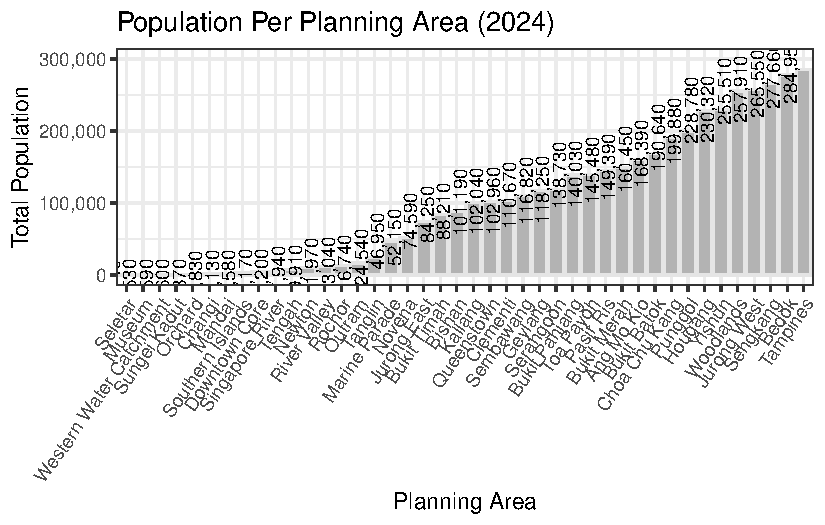
\includegraphics{Take-home_Ex01_files/figure-pdf/unnamed-chunk-8-1.pdf}

\subsection{Insight}\label{insight}

\begin{itemize}
\item
  Plot 1, a bar chart, lists the top 10 most populous planning areas
  (PAs): Tampines (284,950), Bedok (277,660), Sengkang (265,550), Jurong
  West (257,910), Woodlands (255,510), Yishun (230,320), Hougang
  (228,780), Punggol (199,880), Choa Chu Kang (190,640), and Bukit Batok
  (168,390). This highlights Tampines as the densest hub.
\item
  Plot 2, a stacked bar chart, shows total population across all PAs,
  with the top 10 aligning with Plot 1's rankings, peaking at Tampines
  and tapering off in less populated areas like Western Water Catchment.
\item
  Both plots confirm a concentration of population in urban PAs, with a
  clear hierarchy led by Tampines, Bedok, and Sengkang. This indicate a
  need for targeted infrastructure and services in these high-density
  areas, with potential resource allocation challenges in less populated
  regions.
\end{itemize}

\section{4 Distribution of Singapore's Population by Age and
Gender}\label{distribution-of-singapores-population-by-age-and-gender}

\subsection{Plot 1}\label{plot-1-1}

\begin{Shaded}
\begin{Highlighting}[]
\FunctionTok{library}\NormalTok{(ggplot2)}
\FunctionTok{library}\NormalTok{(dplyr)}

\CommentTok{\# Group into 5{-}year bins and summarise}
\NormalTok{pyramid\_data }\OtherTok{\textless{}{-}}\NormalTok{ respopagesex2024 }\SpecialCharTok{\%\textgreater{}\%}
  \FunctionTok{mutate}\NormalTok{(}
    \AttributeTok{Age =} \FunctionTok{as.numeric}\NormalTok{(Age),}
    \AttributeTok{Age\_Group =} \FunctionTok{cut}\NormalTok{(Age,}
                    \AttributeTok{breaks =} \FunctionTok{seq}\NormalTok{(}\DecValTok{0}\NormalTok{, }\DecValTok{100}\NormalTok{, }\AttributeTok{by =} \DecValTok{5}\NormalTok{),}
                    \AttributeTok{labels =} \FunctionTok{paste}\NormalTok{(}\FunctionTok{seq}\NormalTok{(}\DecValTok{0}\NormalTok{, }\DecValTok{95}\NormalTok{, }\AttributeTok{by =} \DecValTok{5}\NormalTok{), }\FunctionTok{seq}\NormalTok{(}\DecValTok{4}\NormalTok{, }\DecValTok{99}\NormalTok{, }\AttributeTok{by =} \DecValTok{5}\NormalTok{), }\AttributeTok{sep =} \StringTok{"{-}"}\NormalTok{),}
                    \AttributeTok{include.lowest =} \ConstantTok{TRUE}\NormalTok{)}
\NormalTok{  ) }\SpecialCharTok{\%\textgreater{}\%}
  \FunctionTok{filter}\NormalTok{(Sex }\SpecialCharTok{\%in\%} \FunctionTok{c}\NormalTok{(}\StringTok{"Males"}\NormalTok{, }\StringTok{"Females"}\NormalTok{)) }\SpecialCharTok{\%\textgreater{}\%}
  \FunctionTok{group\_by}\NormalTok{(Age\_Group, Sex) }\SpecialCharTok{\%\textgreater{}\%}
  \FunctionTok{summarise}\NormalTok{(}\AttributeTok{Total\_Pop =} \FunctionTok{sum}\NormalTok{(Pop, }\AttributeTok{na.rm =} \ConstantTok{TRUE}\NormalTok{), }\AttributeTok{.groups =} \StringTok{"drop"}\NormalTok{) }\SpecialCharTok{\%\textgreater{}\%}
  \FunctionTok{mutate}\NormalTok{(}\AttributeTok{Population =} \FunctionTok{ifelse}\NormalTok{(Sex }\SpecialCharTok{==} \StringTok{"Males"}\NormalTok{, }\SpecialCharTok{{-}}\NormalTok{Total\_Pop, Total\_Pop))}

\CommentTok{\# Ensure proper order for Age\_Group}
\NormalTok{pyramid\_data}\SpecialCharTok{$}\NormalTok{Age\_Group }\OtherTok{\textless{}{-}} \FunctionTok{factor}\NormalTok{(pyramid\_data}\SpecialCharTok{$}\NormalTok{Age\_Group, }\AttributeTok{levels =} \FunctionTok{unique}\NormalTok{(pyramid\_data}\SpecialCharTok{$}\NormalTok{Age\_Group))}

\CommentTok{\# Plot the age pyramid}
\FunctionTok{ggplot}\NormalTok{(pyramid\_data, }\FunctionTok{aes}\NormalTok{(}\AttributeTok{x =}\NormalTok{ Population, }\AttributeTok{y =}\NormalTok{ Age\_Group, }\AttributeTok{fill =}\NormalTok{ Sex)) }\SpecialCharTok{+}
  \FunctionTok{geom\_bar}\NormalTok{(}\AttributeTok{stat =} \StringTok{"identity"}\NormalTok{) }\SpecialCharTok{+}
  \FunctionTok{scale\_x\_continuous}\NormalTok{(}\AttributeTok{labels =}\NormalTok{ abs, }\AttributeTok{name =} \StringTok{"Population"}\NormalTok{) }\SpecialCharTok{+}
  \FunctionTok{scale\_y\_discrete}\NormalTok{(}\AttributeTok{name =} \StringTok{"Age Group"}\NormalTok{) }\SpecialCharTok{+}
  \FunctionTok{scale\_fill\_manual}\NormalTok{(}\AttributeTok{values =} \FunctionTok{c}\NormalTok{(}\StringTok{"Males"} \OtherTok{=} \StringTok{"grey70"}\NormalTok{, }\StringTok{"Females"} \OtherTok{=} \StringTok{"grey90"}\NormalTok{)) }\SpecialCharTok{+}
  \FunctionTok{theme\_bw}\NormalTok{() }\SpecialCharTok{+}
  \FunctionTok{ggtitle}\NormalTok{(}\StringTok{"Singapore Population Pyramid (2024)"}\NormalTok{) }\SpecialCharTok{+}
  \FunctionTok{theme}\NormalTok{(}\AttributeTok{legend.position =} \StringTok{"bottom"}\NormalTok{)}
\end{Highlighting}
\end{Shaded}

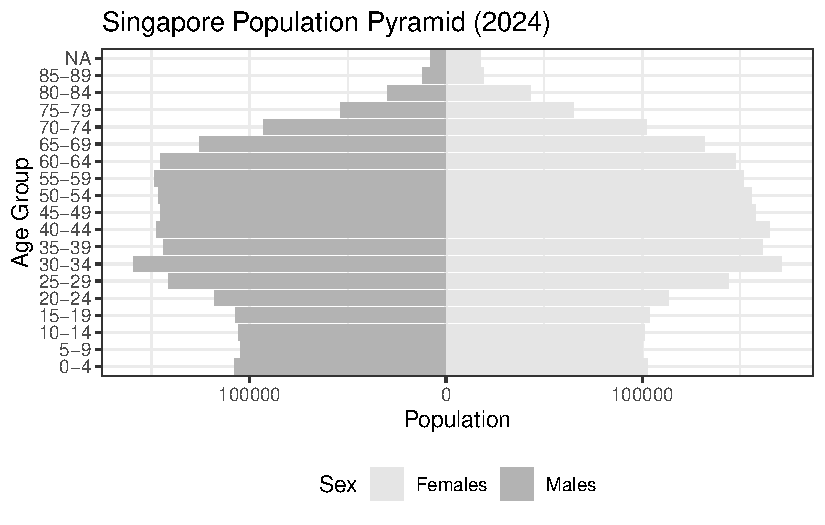
\includegraphics{Take-home_Ex01_files/figure-pdf/unnamed-chunk-9-1.pdf}

\subsection{Plot 2}\label{plot-2-1}

\begin{Shaded}
\begin{Highlighting}[]
\FunctionTok{library}\NormalTok{(readr)}
\FunctionTok{library}\NormalTok{(dplyr)}
\FunctionTok{library}\NormalTok{(ggplot2)}
\FunctionTok{library}\NormalTok{(scales)}

\CommentTok{\# Disable scientific notation}
\FunctionTok{options}\NormalTok{(}\AttributeTok{scipen =} \DecValTok{999}\NormalTok{)}

\CommentTok{\# Load data}
\NormalTok{respopagesex2024 }\OtherTok{\textless{}{-}} \FunctionTok{read\_csv}\NormalTok{(}\StringTok{"TakeHome\_01/respopagesex2024.csv"}\NormalTok{)}

\CommentTok{\# Convert Age Seyfert’s correction for age groups}
\NormalTok{pop\_by\_age }\OtherTok{\textless{}{-}}\NormalTok{ respopagesex2024 }\SpecialCharTok{\%\textgreater{}\%}
  \FunctionTok{mutate}\NormalTok{(}
    \AttributeTok{Pop =} \FunctionTok{as.numeric}\NormalTok{(Pop),}
    \AttributeTok{Age\_Num =} \FunctionTok{case\_when}\NormalTok{(}
\NormalTok{      Age }\SpecialCharTok{==} \StringTok{"90\_and\_Over"} \SpecialCharTok{\textasciitilde{}} \DecValTok{90}\NormalTok{,}
      \ConstantTok{TRUE} \SpecialCharTok{\textasciitilde{}} \FunctionTok{as.numeric}\NormalTok{(}\FunctionTok{gsub}\NormalTok{(}\StringTok{"–.*"}\NormalTok{, }\StringTok{""}\NormalTok{, Age)) }\SpecialCharTok{+} \FloatTok{2.5}  \CommentTok{\# Midpoint of 5{-}year age groups}
\NormalTok{    )}
\NormalTok{  ) }\SpecialCharTok{\%\textgreater{}\%}
  \FunctionTok{filter}\NormalTok{(}\SpecialCharTok{!}\FunctionTok{is.na}\NormalTok{(Pop) }\SpecialCharTok{\&}\NormalTok{ Pop }\SpecialCharTok{\textgreater{}} \DecValTok{0}\NormalTok{)}

\CommentTok{\# Expand data to represent each individual}
\NormalTok{age\_data }\OtherTok{\textless{}{-}}\NormalTok{ pop\_by\_age }\SpecialCharTok{\%\textgreater{}\%}
  \FunctionTok{uncount}\NormalTok{(Pop)  }\CommentTok{\# Repeats each row by Pop value}

\CommentTok{\# Create histogram}
\NormalTok{p }\OtherTok{\textless{}{-}} \FunctionTok{ggplot}\NormalTok{(}\AttributeTok{data =}\NormalTok{ age\_data, }\FunctionTok{aes}\NormalTok{(}\AttributeTok{x =}\NormalTok{ Age\_Num)) }\SpecialCharTok{+}
  \FunctionTok{geom\_histogram}\NormalTok{(}
    \AttributeTok{binwidth =} \DecValTok{5}\NormalTok{,  }\CommentTok{\# 5{-}year age bins}
    \AttributeTok{fill =} \StringTok{"grey70"}\NormalTok{,}
    \AttributeTok{color =} \StringTok{"grey90"}
\NormalTok{  ) }\SpecialCharTok{+}
  \FunctionTok{theme\_bw}\NormalTok{() }\SpecialCharTok{+}
  \FunctionTok{ggtitle}\NormalTok{(}\StringTok{"Age Distribution of Singapore Population, 2024"}\NormalTok{) }\SpecialCharTok{+}
  \FunctionTok{xlab}\NormalTok{(}\StringTok{"Age (Years)"}\NormalTok{) }\SpecialCharTok{+}
  \FunctionTok{ylab}\NormalTok{(}\StringTok{"Population"}\NormalTok{) }\SpecialCharTok{+}
  \FunctionTok{scale\_x\_continuous}\NormalTok{(}
    \AttributeTok{breaks =} \FunctionTok{seq}\NormalTok{(}\DecValTok{0}\NormalTok{, }\DecValTok{100}\NormalTok{, }\AttributeTok{by =} \DecValTok{10}\NormalTok{),}
    \AttributeTok{limits =} \FunctionTok{c}\NormalTok{(}\DecValTok{0}\NormalTok{, }\DecValTok{100}\NormalTok{)}
\NormalTok{  ) }\SpecialCharTok{+}
  \FunctionTok{scale\_y\_continuous}\NormalTok{(}\AttributeTok{labels =}\NormalTok{ comma)}

\CommentTok{\# Render plot}
\FunctionTok{print}\NormalTok{(p)}
\end{Highlighting}
\end{Shaded}

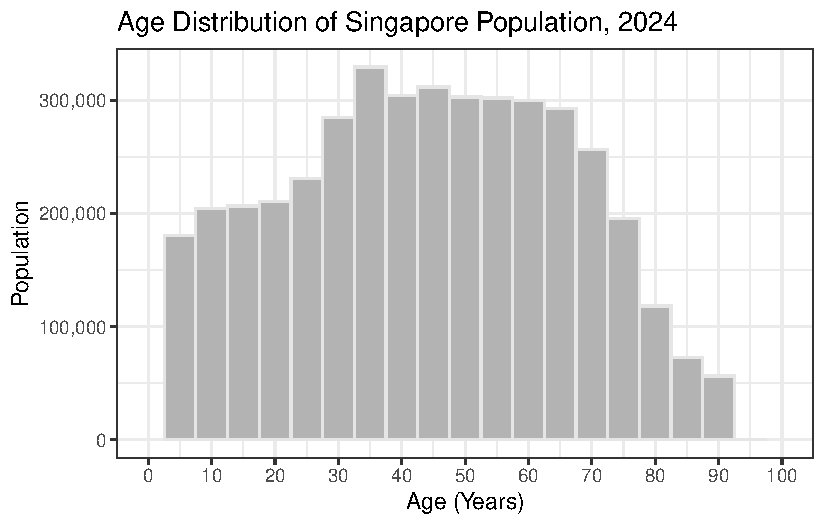
\includegraphics{Take-home_Ex01_files/figure-pdf/unnamed-chunk-10-1.pdf}

\subsection{Insight}\label{insight-1}

\begin{itemize}
\item
  Plot 1, a population pyramid, shows the age and gender distribution
  across the entire population, with a broad working-age base (30--59),
  a smaller youth (0--19), and aN elderly group (60--80+). Females
  slightly outnumber males in the 70+ age groups, reflecting higher life
  expectancy.
\item
  Plot 2, a histogram, displays the overall age distribution, confirming
  the working-age peak (30--50 years), a small youth population, and a
  gradual increase in elderly (60--80+), with a slight female skew in
  older ages.
\item
  Together, they highlight Singapore's aging population, with a
  shrinking youth base, a dominant working-age group, and a gender
  imbalance in the elderly (more females). This indicate a need for
  eldercare (especially for females), workforce support, and policies to
  address low birth rates.
\end{itemize}

\section{5 Distribution of Population and Age Across Top Five Planning
Areas by Gender and Age
Group}\label{distribution-of-population-and-age-across-top-five-planning-areas-by-gender-and-age-group}

\subsection{Plot 1}\label{plot-1-2}

\begin{Shaded}
\begin{Highlighting}[]
\FunctionTok{library}\NormalTok{(readr)}
\FunctionTok{library}\NormalTok{(dplyr)}
\FunctionTok{library}\NormalTok{(ggplot2)}
\FunctionTok{library}\NormalTok{(scales)}

\CommentTok{\# Disable scientific notation}
\FunctionTok{options}\NormalTok{(}\AttributeTok{scipen =} \DecValTok{999}\NormalTok{)}

\CommentTok{\# Load data}
\NormalTok{respopagesex2024 }\OtherTok{\textless{}{-}} \FunctionTok{read\_csv}\NormalTok{(}\StringTok{"TakeHome\_01/respopagesex2024.csv"}\NormalTok{)}

\CommentTok{\# Create age groups}
\NormalTok{pop\_by\_pa\_age }\OtherTok{\textless{}{-}}\NormalTok{ respopagesex2024 }\SpecialCharTok{\%\textgreater{}\%}
  \FunctionTok{mutate}\NormalTok{(}
    \AttributeTok{Pop =} \FunctionTok{as.numeric}\NormalTok{(Pop),}
    \AttributeTok{Age =} \FunctionTok{ifelse}\NormalTok{(Age }\SpecialCharTok{==} \StringTok{"90\_and\_Over"}\NormalTok{, }\DecValTok{90}\NormalTok{, }\FunctionTok{as.numeric}\NormalTok{(Age)),}
    \AttributeTok{Age\_Group =} \FunctionTok{case\_when}\NormalTok{(}
\NormalTok{      Age }\SpecialCharTok{\textless{}=} \DecValTok{19} \SpecialCharTok{\textasciitilde{}} \StringTok{"0–19"}\NormalTok{,}
\NormalTok{      Age }\SpecialCharTok{\textless{}=} \DecValTok{39} \SpecialCharTok{\textasciitilde{}} \StringTok{"20–39"}\NormalTok{,}
\NormalTok{      Age }\SpecialCharTok{\textless{}=} \DecValTok{59} \SpecialCharTok{\textasciitilde{}} \StringTok{"40–59"}\NormalTok{,}
\NormalTok{      Age }\SpecialCharTok{\textless{}=} \DecValTok{79} \SpecialCharTok{\textasciitilde{}} \StringTok{"60–79"}\NormalTok{,}
      \ConstantTok{TRUE} \SpecialCharTok{\textasciitilde{}} \StringTok{"80+"}
\NormalTok{    )}
\NormalTok{  ) }\SpecialCharTok{\%\textgreater{}\%}
  \FunctionTok{filter}\NormalTok{(}\SpecialCharTok{!}\FunctionTok{is.na}\NormalTok{(Pop) }\SpecialCharTok{\&}\NormalTok{ Pop }\SpecialCharTok{\textgreater{}} \DecValTok{0}\NormalTok{) }\SpecialCharTok{\%\textgreater{}\%}
  \FunctionTok{group\_by}\NormalTok{(PA, Age\_Group) }\SpecialCharTok{\%\textgreater{}\%}
  \FunctionTok{summarise}\NormalTok{(}
    \AttributeTok{Pop =} \FunctionTok{sum}\NormalTok{(Pop, }\AttributeTok{na.rm =} \ConstantTok{TRUE}\NormalTok{),}
    \AttributeTok{Num\_Subzones =} \FunctionTok{n\_distinct}\NormalTok{(SZ)}
\NormalTok{  ) }\SpecialCharTok{\%\textgreater{}\%}
  \FunctionTok{ungroup}\NormalTok{()}

\CommentTok{\# Calculate total population per PA for ordering and select top 10}
\NormalTok{pa\_order }\OtherTok{\textless{}{-}}\NormalTok{ pop\_by\_pa\_age }\SpecialCharTok{\%\textgreater{}\%}
  \FunctionTok{group\_by}\NormalTok{(PA) }\SpecialCharTok{\%\textgreater{}\%}
  \FunctionTok{summarise}\NormalTok{(}\AttributeTok{Total\_Pop =} \FunctionTok{sum}\NormalTok{(Pop)) }\SpecialCharTok{\%\textgreater{}\%}
  \FunctionTok{arrange}\NormalTok{(}\FunctionTok{desc}\NormalTok{(Total\_Pop)) }\SpecialCharTok{\%\textgreater{}\%}
  \FunctionTok{slice\_head}\NormalTok{(}\AttributeTok{n =} \DecValTok{5}\NormalTok{)}

\CommentTok{\# Filter data to top 10 PAs}
\NormalTok{pop\_by\_pa\_age }\OtherTok{\textless{}{-}}\NormalTok{ pop\_by\_pa\_age }\SpecialCharTok{\%\textgreater{}\%}
  \FunctionTok{filter}\NormalTok{(PA }\SpecialCharTok{\%in\%}\NormalTok{ pa\_order}\SpecialCharTok{$}\NormalTok{PA)}

\CommentTok{\# Add total population}
\NormalTok{pop\_by\_pa\_age }\OtherTok{\textless{}{-}}\NormalTok{ pop\_by\_pa\_age }\SpecialCharTok{\%\textgreater{}\%}
  \FunctionTok{left\_join}\NormalTok{(pa\_order, }\AttributeTok{by =} \StringTok{"PA"}\NormalTok{)}

\CommentTok{\# Create stacked bar chart}
\NormalTok{p1 }\OtherTok{\textless{}{-}} \FunctionTok{ggplot}\NormalTok{(}\AttributeTok{data =}\NormalTok{ pop\_by\_pa\_age, }\FunctionTok{aes}\NormalTok{(}\AttributeTok{x =} \FunctionTok{reorder}\NormalTok{(PA, Total\_Pop), }\AttributeTok{y =}\NormalTok{ Pop, }\AttributeTok{fill =}\NormalTok{ Age\_Group)) }\SpecialCharTok{+}
  \FunctionTok{geom\_bar}\NormalTok{(}
    \AttributeTok{stat =} \StringTok{"identity"}\NormalTok{,}
    \AttributeTok{position =} \StringTok{"stack"}  \CommentTok{\# Stacked bars}
\NormalTok{  ) }\SpecialCharTok{+}
  \FunctionTok{theme\_bw}\NormalTok{() }\SpecialCharTok{+}
  \FunctionTok{ggtitle}\NormalTok{(}\StringTok{"Population by Top 5 Planning Areas and Age Group, Singapore 2024"}\NormalTok{) }\SpecialCharTok{+}
  \FunctionTok{xlab}\NormalTok{(}\StringTok{"Planning Area"}\NormalTok{) }\SpecialCharTok{+}
  \FunctionTok{ylab}\NormalTok{(}\StringTok{"Population"}\NormalTok{) }\SpecialCharTok{+}
  \FunctionTok{theme}\NormalTok{(}
    \AttributeTok{axis.text.x =} \FunctionTok{element\_text}\NormalTok{(}\AttributeTok{angle =} \DecValTok{55}\NormalTok{, }\AttributeTok{hjust =} \DecValTok{1}\NormalTok{)}
\NormalTok{  ) }\SpecialCharTok{+}
  \FunctionTok{scale\_y\_continuous}\NormalTok{(}
    \AttributeTok{labels =}\NormalTok{ comma,}
    \AttributeTok{breaks =} \FunctionTok{seq}\NormalTok{(}\DecValTok{0}\NormalTok{, }\FunctionTok{ceiling}\NormalTok{(}\FunctionTok{max}\NormalTok{(pa\_order}\SpecialCharTok{$}\NormalTok{Total\_Pop, }\AttributeTok{na.rm =} \ConstantTok{TRUE}\NormalTok{) }\SpecialCharTok{/} \DecValTok{100000}\NormalTok{) }\SpecialCharTok{*} \DecValTok{100000}\NormalTok{, }\AttributeTok{by =} \DecValTok{100000}\NormalTok{),}
    \AttributeTok{limits =} \FunctionTok{c}\NormalTok{(}\DecValTok{0}\NormalTok{, }\FunctionTok{ceiling}\NormalTok{(}\FunctionTok{max}\NormalTok{(pa\_order}\SpecialCharTok{$}\NormalTok{Total\_Pop, }\AttributeTok{na.rm =} \ConstantTok{TRUE}\NormalTok{) }\SpecialCharTok{/} \DecValTok{100000}\NormalTok{) }\SpecialCharTok{*} \DecValTok{100000}\NormalTok{)}
\NormalTok{  ) }\SpecialCharTok{+}
  \FunctionTok{scale\_fill\_manual}\NormalTok{(}\AttributeTok{values =} \FunctionTok{c}\NormalTok{(}\StringTok{"0–19"} \OtherTok{=} \StringTok{"grey95"}\NormalTok{, }\StringTok{"20–39"} \OtherTok{=} \StringTok{"grey80"}\NormalTok{, }\StringTok{"40–59"} \OtherTok{=} \StringTok{"grey65"}\NormalTok{, }\StringTok{"60–79"} \OtherTok{=} \StringTok{"grey50"}\NormalTok{, }\StringTok{"80+"} \OtherTok{=} \StringTok{"grey35"}\NormalTok{))}

\CommentTok{\# Render plot}
\FunctionTok{print}\NormalTok{(p1)}
\end{Highlighting}
\end{Shaded}

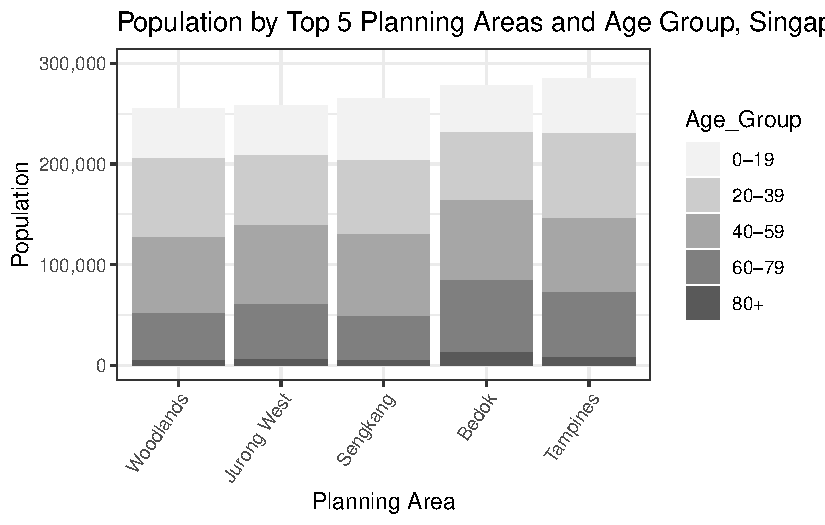
\includegraphics{Take-home_Ex01_files/figure-pdf/unnamed-chunk-11-1.pdf}

\subsection{Plot 2}\label{plot-2-2}

\begin{Shaded}
\begin{Highlighting}[]
\FunctionTok{library}\NormalTok{(readr)}
\FunctionTok{library}\NormalTok{(dplyr)}
\FunctionTok{library}\NormalTok{(ggplot2)}
\FunctionTok{library}\NormalTok{(scales)}
\FunctionTok{library}\NormalTok{(ggridges)}

\CommentTok{\# Disable scientific notation}
\FunctionTok{options}\NormalTok{(}\AttributeTok{scipen =} \DecValTok{999}\NormalTok{)}

\CommentTok{\# Load data}
\NormalTok{respopagesex2024 }\OtherTok{\textless{}{-}} \FunctionTok{read\_csv}\NormalTok{(}\StringTok{"TakeHome\_01/respopagesex2024.csv"}\NormalTok{)}

\CommentTok{\# Prepare data: Convert Age to numeric}
\NormalTok{pop\_data }\OtherTok{\textless{}{-}}\NormalTok{ respopagesex2024 }\SpecialCharTok{\%\textgreater{}\%}
  \FunctionTok{mutate}\NormalTok{(}
    \AttributeTok{Pop =} \FunctionTok{as.numeric}\NormalTok{(Pop),}
    \AttributeTok{Age\_Num =} \FunctionTok{case\_when}\NormalTok{(}
\NormalTok{      Age }\SpecialCharTok{==} \StringTok{"90\_and\_Over"} \SpecialCharTok{\textasciitilde{}} \DecValTok{90}\NormalTok{,}
      \ConstantTok{TRUE} \SpecialCharTok{\textasciitilde{}} \FunctionTok{as.numeric}\NormalTok{(}\FunctionTok{gsub}\NormalTok{(}\StringTok{"–.*"}\NormalTok{, }\StringTok{""}\NormalTok{, Age)) }\SpecialCharTok{+} \FloatTok{2.5}  \CommentTok{\# Midpoint of 5{-}year age groups}
\NormalTok{    )}
\NormalTok{  ) }\SpecialCharTok{\%\textgreater{}\%}
  \FunctionTok{filter}\NormalTok{(}\SpecialCharTok{!}\FunctionTok{is.na}\NormalTok{(Pop) }\SpecialCharTok{\&}\NormalTok{ Pop }\SpecialCharTok{\textgreater{}} \DecValTok{0} \SpecialCharTok{\&} \SpecialCharTok{!}\FunctionTok{is.na}\NormalTok{(Age\_Num))}

\CommentTok{\# Order PAs by total population and select top 10}
\NormalTok{pa\_order }\OtherTok{\textless{}{-}}\NormalTok{ pop\_data }\SpecialCharTok{\%\textgreater{}\%}
  \FunctionTok{group\_by}\NormalTok{(PA) }\SpecialCharTok{\%\textgreater{}\%}
  \FunctionTok{summarise}\NormalTok{(}\AttributeTok{Total\_Pop =} \FunctionTok{sum}\NormalTok{(Pop, }\AttributeTok{na.rm =} \ConstantTok{TRUE}\NormalTok{)) }\SpecialCharTok{\%\textgreater{}\%}
  \FunctionTok{arrange}\NormalTok{(}\FunctionTok{desc}\NormalTok{(Total\_Pop)) }\SpecialCharTok{\%\textgreater{}\%}
  \FunctionTok{slice\_head}\NormalTok{(}\AttributeTok{n =} \DecValTok{5}\NormalTok{) }\SpecialCharTok{\%\textgreater{}\%}
  \FunctionTok{pull}\NormalTok{(PA)}

\CommentTok{\# Filter data to top 10 PAs}
\NormalTok{age\_data }\OtherTok{\textless{}{-}}\NormalTok{ pop\_data }\SpecialCharTok{\%\textgreater{}\%}
  \FunctionTok{filter}\NormalTok{(PA }\SpecialCharTok{\%in\%}\NormalTok{ pa\_order) }\SpecialCharTok{\%\textgreater{}\%}
  \FunctionTok{uncount}\NormalTok{(Pop)  }\CommentTok{\# Expand data to represent each individual (weighted by Pop)}

\CommentTok{\# Create ridgeline plot}
\NormalTok{p2 }\OtherTok{\textless{}{-}} \FunctionTok{ggplot}\NormalTok{(}\AttributeTok{data =}\NormalTok{ age\_data, }\FunctionTok{aes}\NormalTok{(}\AttributeTok{x =}\NormalTok{ Age\_Num, }\AttributeTok{y =} \FunctionTok{factor}\NormalTok{(PA, }\AttributeTok{levels =} \FunctionTok{rev}\NormalTok{(pa\_order)), }\AttributeTok{height =}\NormalTok{ ..density..)) }\SpecialCharTok{+}
  \FunctionTok{geom\_density\_ridges}\NormalTok{(}
    \AttributeTok{stat =} \StringTok{"density"}\NormalTok{,}
    \AttributeTok{fill =} \StringTok{"grey20"}\NormalTok{,}
    \AttributeTok{color =} \StringTok{"grey90"}\NormalTok{,}
    \AttributeTok{scale =} \FloatTok{1.5}\NormalTok{,  }\CommentTok{\# Controls ridge overlap}
    \AttributeTok{alpha =} \FloatTok{1.5}
\NormalTok{  ) }\SpecialCharTok{+}
  \FunctionTok{facet\_wrap}\NormalTok{(}\SpecialCharTok{\textasciitilde{}}\NormalTok{ Sex, }\AttributeTok{ncol =} \DecValTok{2}\NormalTok{) }\SpecialCharTok{+}
  \FunctionTok{theme\_bw}\NormalTok{() }\SpecialCharTok{+}
  \FunctionTok{ggtitle}\NormalTok{(}\StringTok{"Age Distribution in Top 5 Populated Planning Areas by Gender, Singapore 2024"}\NormalTok{) }\SpecialCharTok{+}
  \FunctionTok{xlab}\NormalTok{(}\StringTok{"Age (Years)"}\NormalTok{) }\SpecialCharTok{+}
  \FunctionTok{ylab}\NormalTok{(}\StringTok{"Planning Area"}\NormalTok{) }\SpecialCharTok{+}
  \FunctionTok{scale\_x\_continuous}\NormalTok{(}
    \AttributeTok{breaks =} \FunctionTok{seq}\NormalTok{(}\DecValTok{0}\NormalTok{, }\DecValTok{100}\NormalTok{, }\AttributeTok{by =} \DecValTok{20}\NormalTok{),}
    \AttributeTok{limits =} \FunctionTok{c}\NormalTok{(}\DecValTok{0}\NormalTok{, }\DecValTok{100}\NormalTok{)}
\NormalTok{  ) }\SpecialCharTok{+}
  \FunctionTok{theme}\NormalTok{(}
    \AttributeTok{axis.text.y =} \FunctionTok{element\_text}\NormalTok{(}\AttributeTok{size =} \DecValTok{12}\NormalTok{),  }\CommentTok{\# Larger text for fewer PAs}
    \AttributeTok{axis.text.x =} \FunctionTok{element\_text}\NormalTok{(}\AttributeTok{size =} \DecValTok{12}\NormalTok{),}
    \AttributeTok{axis.title =} \FunctionTok{element\_text}\NormalTok{(}\AttributeTok{size =} \DecValTok{12}\NormalTok{),}
    \AttributeTok{plot.title =} \FunctionTok{element\_text}\NormalTok{(}\AttributeTok{size =} \DecValTok{15}\NormalTok{),}
    \AttributeTok{strip.text =} \FunctionTok{element\_text}\NormalTok{(}\AttributeTok{size =} \DecValTok{12}\NormalTok{),}
    \AttributeTok{strip.background =} \FunctionTok{element\_rect}\NormalTok{(}\AttributeTok{fill =} \StringTok{"grey90"}\NormalTok{)}
\NormalTok{  )}

\CommentTok{\# Render plot}
\FunctionTok{print}\NormalTok{(p2)}
\end{Highlighting}
\end{Shaded}

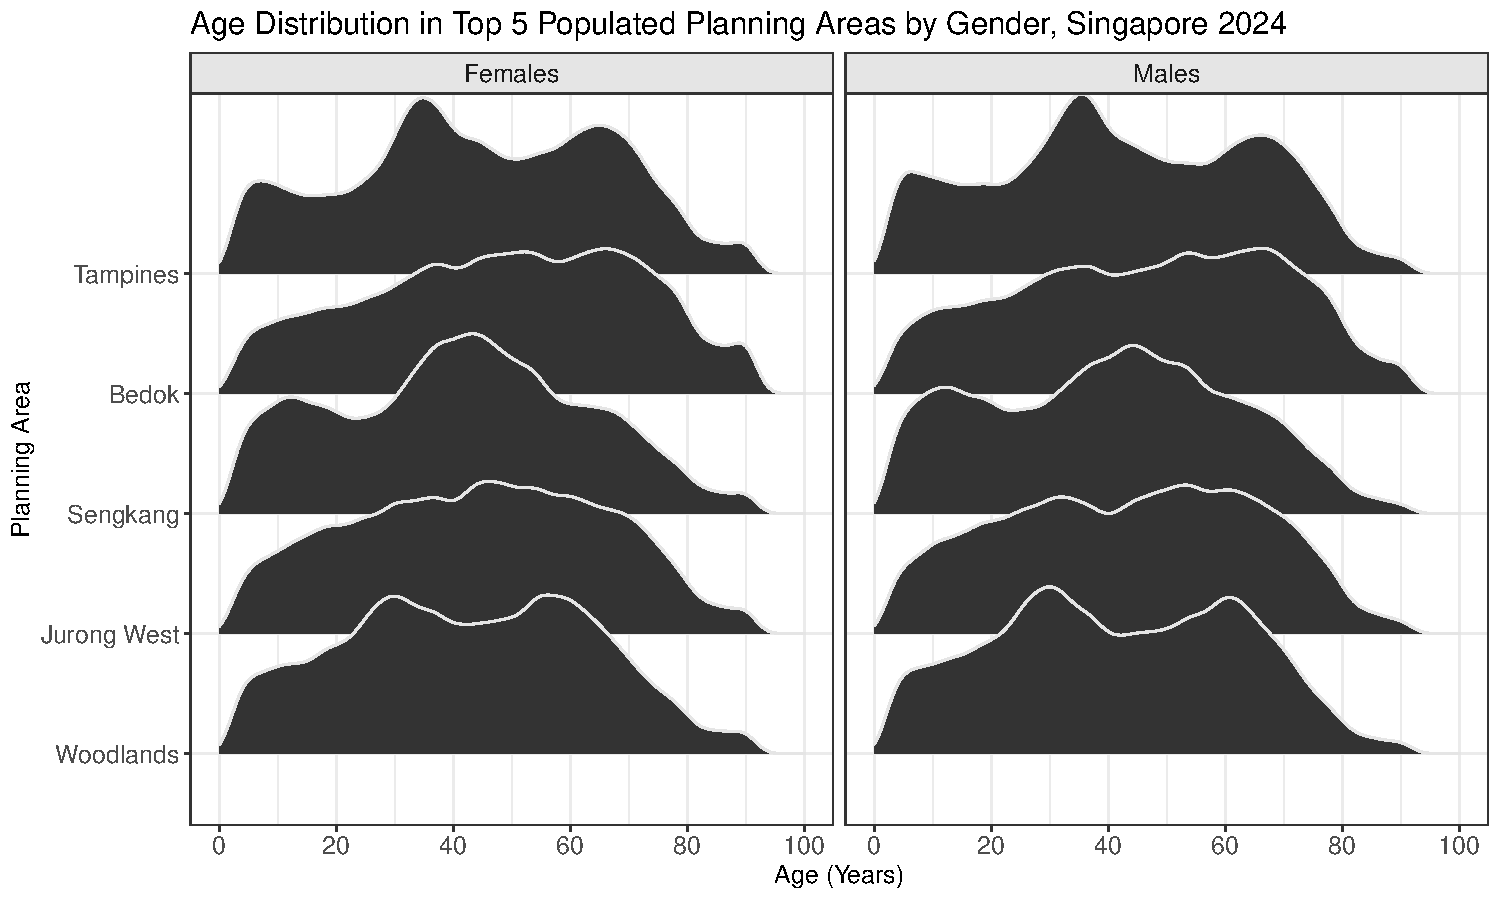
\includegraphics{Take-home_Ex01_files/figure-pdf/unnamed-chunk-12-1.pdf}

\subsection{Insight}\label{insight-2}

\begin{itemize}
\item
  Both plots provide insights into Singapore's 2024 population across
  the top 5 planning areas (PAs): Tampines, Bedok, Sengkang, Jurong
  West, and Woodlands.
\item
  The stacked bar chart (Plot 1) shows Tampines as the most populous
  (300,000), with a dominant working-age group (20--59) across all PAs,
  a small youth group (0--19), and notable elderly groups (60--80+) in
  Bedok and Woodlands.
\item
  The ridgeline plot (Plot 2) confirms these trends, highlighting
  working-age peaks at 30--50, a young peak in Sengkang (0--20), and
  broader elderly curves in Bedok and Woodlands.
\item
  Gender-wise, females show higher elderly presence (60--80+), while
  males peak at 30--50. Sengkang is likely family-oriented, while Bedok
  and Woodlands are aging, and Tampines and Jurong West are balanced.
\end{itemize}

\section{6 Summary and Conclusion}\label{summary-and-conclusion}

This project visually explores Singapore's 2024 resident population
using official demographic data to highlight trends in age, gender, and
regional distribution.

Key findings:

\begin{itemize}
\item
  \textbf{Urban areas are densely populated}: The top 10 planning zones
  Tampines, Bedok, and Sengkang hold a large share of residents,
  creating demands for infrastructure.
\item
  \textbf{Age and gender patterns}: Most people fall within the
  working-age group (30--59), with fewer young residents and a rising
  elderly population (especially women), reflecting longer life
  expectancy.
\item
  \textbf{Regional differences}: Each area has unique demographics
  Sengkang has a younger population, Bedok and Woodlands have more
  elderly residents, and Tampines and Jurong West are more balanced.
\end{itemize}

Overall, Singapore's population is aging, with varying needs across
regions. Policymakers should adapt by improving eldercare in aging
areas, supporting youth and families where needed, and scaling public
services in crowded districts. These visuals can help people understand
these trends and guide decisions in urban planning, healthcare, and
social services.

\section{7 References}\label{references}

\href{https://ggplot2.tidyverse.org//index.html}{Create Elegant Data
Visualisations Using the Grammar of Graphics • ggplot2}

\href{https://quarto.org/}{Quarto}

\href{https://clauswilke.com/dataviz/}{Fundamentals of Data
Visualization}

\section{8 Take Home Exercise 1 (Part
2)}\label{take-home-exercise-1-part-2}

\section{8.1 Task}\label{task}

Selecting one submission provided by your classmate, critic three good
design principles and three areas for further improvement. With
reference to the comment, prepare the makeover version of the data
visualisation.

\section{8.2 Class mate original plot}\label{class-mate-original-plot}

\subsection{View Column Names and Adjust
Data}\label{view-column-names-and-adjust-data}

\begin{Shaded}
\begin{Highlighting}[]
\FunctionTok{colnames}\NormalTok{(respopagesex2024)}
\end{Highlighting}
\end{Shaded}

\begin{verbatim}
[1] "PA"   "SZ"   "Age"  "Sex"  "Pop"  "Time"
\end{verbatim}

\begin{Shaded}
\begin{Highlighting}[]
\NormalTok{df }\OtherTok{\textless{}{-}} \FunctionTok{tibble}\NormalTok{(}
  \AttributeTok{PA =} \FunctionTok{c}\NormalTok{(}\StringTok{"Planning Area"}\NormalTok{),}
  \AttributeTok{SZ =} \FunctionTok{c}\NormalTok{(}\StringTok{"Subzone"}\NormalTok{),}
  \AttributeTok{Age =} \FunctionTok{c}\NormalTok{(}\StringTok{"Age"}\NormalTok{),}
  \AttributeTok{Sex =} \FunctionTok{c}\NormalTok{(}\StringTok{"Sex"}\NormalTok{),}
  \AttributeTok{Pop =} \FunctionTok{c}\NormalTok{(}\StringTok{"Population"}\NormalTok{),}
  \AttributeTok{Time =} \FunctionTok{c}\NormalTok{(}\StringTok{"Time"}\NormalTok{)}
\NormalTok{)}

\NormalTok{df }\SpecialCharTok{\%\textgreater{}\%}
\NormalTok{  knitr}\SpecialCharTok{::}\FunctionTok{kable}\NormalTok{(}\AttributeTok{caption =} \StringTok{"Column Information"}\NormalTok{)}
\end{Highlighting}
\end{Shaded}

\begin{longtable}[]{@{}llllll@{}}
\caption{Column Information}\tabularnewline
\toprule\noalign{}
PA & SZ & Age & Sex & Pop & Time \\
\midrule\noalign{}
\endfirsthead
\toprule\noalign{}
PA & SZ & Age & Sex & Pop & Time \\
\midrule\noalign{}
\endhead
\bottomrule\noalign{}
\endlastfoot
Planning Area & Subzone & Age & Sex & Population & Time \\
\end{longtable}

\begin{Shaded}
\begin{Highlighting}[]
\FunctionTok{library}\NormalTok{(dplyr)}

\NormalTok{df\_percent }\OtherTok{\textless{}{-}}\NormalTok{ respopagesex2024 }\SpecialCharTok{\%\textgreater{}\%}
  \FunctionTok{mutate}\NormalTok{(}
    \AttributeTok{Age =} \FunctionTok{as.numeric}\NormalTok{(Age),}
    \AttributeTok{AgeGroup =} \FunctionTok{case\_when}\NormalTok{(}
\NormalTok{      Age }\SpecialCharTok{\textless{}=} \DecValTok{14} \SpecialCharTok{\textasciitilde{}} \StringTok{"Children"}\NormalTok{,}
\NormalTok{      Age }\SpecialCharTok{\textgreater{}=} \DecValTok{15} \SpecialCharTok{\&}\NormalTok{ Age }\SpecialCharTok{\textless{}=} \DecValTok{64} \SpecialCharTok{\textasciitilde{}} \StringTok{"Adults"}\NormalTok{,}
\NormalTok{      Age }\SpecialCharTok{\textgreater{}=} \DecValTok{65} \SpecialCharTok{\textasciitilde{}} \StringTok{"Seniors"}\NormalTok{,}
      \ConstantTok{TRUE} \SpecialCharTok{\textasciitilde{}} \ConstantTok{NA\_character\_}
\NormalTok{    )}
\NormalTok{  ) }\SpecialCharTok{\%\textgreater{}\%}
  \FunctionTok{group\_by}\NormalTok{(PA, AgeGroup) }\SpecialCharTok{\%\textgreater{}\%}
  \FunctionTok{summarise}\NormalTok{(}\AttributeTok{Population =} \FunctionTok{sum}\NormalTok{(Pop), }\AttributeTok{.groups =} \StringTok{"drop"}\NormalTok{) }\SpecialCharTok{\%\textgreater{}\%}
  \FunctionTok{group\_by}\NormalTok{(PA) }\SpecialCharTok{\%\textgreater{}\%}
  \FunctionTok{mutate}\NormalTok{(}
    \AttributeTok{Total\_Pop =} \FunctionTok{sum}\NormalTok{(Population),}
    \AttributeTok{Percent =}\NormalTok{ Population }\SpecialCharTok{/}\NormalTok{ Total\_Pop }\SpecialCharTok{*} \DecValTok{100}
\NormalTok{  )}
\end{Highlighting}
\end{Shaded}

\begin{Shaded}
\begin{Highlighting}[]
\NormalTok{df\_summary }\OtherTok{\textless{}{-}}\NormalTok{ df\_clean }\SpecialCharTok{\%\textgreater{}\%}
  \FunctionTok{group\_by}\NormalTok{(PA) }\SpecialCharTok{\%\textgreater{}\%}
  \FunctionTok{summarise}\NormalTok{(}
    \AttributeTok{Total\_Pop =} \FunctionTok{sum}\NormalTok{(Pop, }\AttributeTok{na.rm =} \ConstantTok{TRUE}\NormalTok{),}
    \AttributeTok{.groups =} \StringTok{"drop"}
\NormalTok{  ) }\SpecialCharTok{\%\textgreater{}\%}
  \FunctionTok{arrange}\NormalTok{(}\FunctionTok{desc}\NormalTok{(Total\_Pop))}
\end{Highlighting}
\end{Shaded}

\subsection{Plot}\label{plot}

\begin{Shaded}
\begin{Highlighting}[]
\NormalTok{bottom10\_pa }\OtherTok{\textless{}{-}}\NormalTok{ df\_summary }\SpecialCharTok{\%\textgreater{}\%}
  \FunctionTok{slice\_min}\NormalTok{(Total\_Pop, }\AttributeTok{n =} \DecValTok{10}\NormalTok{) }\SpecialCharTok{\%\textgreater{}\%}
  \FunctionTok{pull}\NormalTok{(PA)}

\NormalTok{df\_summary\_filtered }\OtherTok{\textless{}{-}}\NormalTok{ df\_summary }\SpecialCharTok{\%\textgreater{}\%}
  \FunctionTok{filter}\NormalTok{(}\SpecialCharTok{!}\NormalTok{PA }\SpecialCharTok{\%in\%}\NormalTok{ bottom10\_pa)}

\FunctionTok{ggplot}\NormalTok{(df\_summary\_filtered, }\FunctionTok{aes}\NormalTok{(}\AttributeTok{x =} \FunctionTok{reorder}\NormalTok{(PA, }\SpecialCharTok{{-}}\NormalTok{Total\_Pop), }\AttributeTok{y =}\NormalTok{ Total\_Pop)) }\SpecialCharTok{+}
  \FunctionTok{geom\_bar}\NormalTok{(}\AttributeTok{stat =} \StringTok{"identity"}\NormalTok{, }\AttributeTok{color =} \StringTok{"black"}\NormalTok{, }\AttributeTok{fill =} \StringTok{"lightblue"}\NormalTok{, }\AttributeTok{width =} \FloatTok{0.75}\NormalTok{) }\SpecialCharTok{+}
  \FunctionTok{scale\_y\_continuous}\NormalTok{(}\AttributeTok{labels =}\NormalTok{ scales}\SpecialCharTok{::}\NormalTok{comma, }\AttributeTok{expand =} \FunctionTok{c}\NormalTok{(}\DecValTok{0}\NormalTok{, }\DecValTok{0}\NormalTok{)) }\SpecialCharTok{+}  
  \FunctionTok{labs}\NormalTok{(}
    \AttributeTok{x =} \StringTok{"Planning Area"}\NormalTok{,}
    \AttributeTok{y =} \StringTok{"Total Population"}\NormalTok{,}
    \AttributeTok{title =} \StringTok{"Total Population by Planning Area (2024)"}
\NormalTok{  ) }\SpecialCharTok{+}
  \FunctionTok{theme\_classic}\NormalTok{(}\AttributeTok{base\_size =} \DecValTok{12}\NormalTok{) }\SpecialCharTok{+}
  \FunctionTok{theme}\NormalTok{(}\AttributeTok{axis.text.x =} \FunctionTok{element\_text}\NormalTok{(}\AttributeTok{angle =} \DecValTok{55}\NormalTok{, }\AttributeTok{hjust =} \DecValTok{1}\NormalTok{))}
\end{Highlighting}
\end{Shaded}

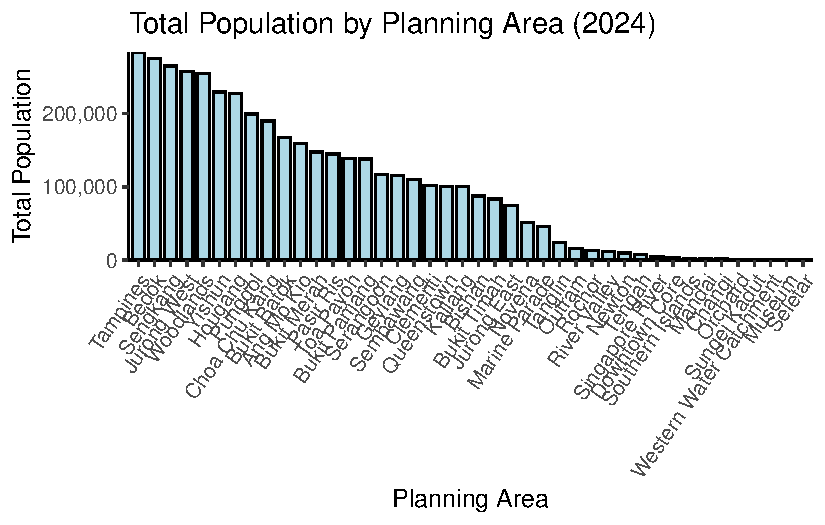
\includegraphics{Take-home_Ex01_files/figure-pdf/unnamed-chunk-21-1.pdf}

\section{8.3 Three Good Design Principles from the
Plot}\label{three-good-design-principles-from-the-plot}

\begin{enumerate}
\def\labelenumi{\arabic{enumi}.}
\tightlist
\item
  Clear Use of Ordering to Enhance Comparison
\end{enumerate}

\begin{itemize}
\tightlist
\item
  Reordering planning areas by descending total population makes it easy
  to compare across areas, aligning with principle of sorting in order
  for clarity in bar charts.
\end{itemize}

\begin{enumerate}
\def\labelenumi{\arabic{enumi}.}
\setcounter{enumi}{1}
\tightlist
\item
  Strong Axis Labels and Title
\end{enumerate}

\begin{itemize}
\item
  The chart uses clear, readable labels and a descriptive title (``Total
  Population by Planning Area (2024)''), fulfilling Wilke's principle
  that charts should be self-explanatory without additional context.
\item
  Fundamentals of Data Visualization -
  \url{https://clauswilke.com/dataviz/}
\end{itemize}

\begin{enumerate}
\def\labelenumi{\arabic{enumi}.}
\setcounter{enumi}{2}
\tightlist
\item
  Good Use of Color and Simplicity
\end{enumerate}

\begin{itemize}
\tightlist
\item
  Light blue fill and black borders provide clear visual contrast
  without being complex to read.
\end{itemize}

\section{8.4 Three Areas that could be
improved}\label{three-areas-that-could-be-improved}

\begin{enumerate}
\def\labelenumi{\arabic{enumi}.}
\tightlist
\item
  Overcrowded X-Axis Labels
\end{enumerate}

\begin{itemize}
\tightlist
\item
  The 45°-rotated text is still hard to read due to the large number of
  planning areas. This decreases clarity. It could improve by switching
  to a horizontal bar chart, especially for ranked data with long
  labels.
\end{itemize}

\begin{enumerate}
\def\labelenumi{\arabic{enumi}.}
\setcounter{enumi}{1}
\tightlist
\item
  No Indication of Units on the Y-Axis
\end{enumerate}

\begin{itemize}
\tightlist
\item
  The y-axis is labeled ``Total Population'' but doesn't specify units.
  Improving it to ``Total Population (number of people)'' can adds
  clarity.
\end{itemize}

\begin{enumerate}
\def\labelenumi{\arabic{enumi}.}
\setcounter{enumi}{2}
\tightlist
\item
  Inefficient Use of Vertical Space
\end{enumerate}

\begin{itemize}
\tightlist
\item
  The chart uses a lot of horizontal space while squeezing the bars
  vertically. In this case, a horizontal layout (coord\_flip) would
  better fit long categorical labels and allow taller bars for clearer
  visual impact.
\end{itemize}

\section{8.5 Makeover version}\label{makeover-version}

\begin{itemize}
\item
  Highlighted the Top 3 most populated planning areas
\item
  Added a subtitle for insight
\item
  Added population for each area for information
\item
  Kept a clean layout with horizontal bars
\end{itemize}

\begin{Shaded}
\begin{Highlighting}[]
\FunctionTok{library}\NormalTok{(dplyr)}
\FunctionTok{library}\NormalTok{(ggplot2)}
\FunctionTok{library}\NormalTok{(scales)}

\NormalTok{df\_highlighted }\OtherTok{\textless{}{-}}\NormalTok{ df\_summary\_filtered }\SpecialCharTok{\%\textgreater{}\%}
  \FunctionTok{mutate}\NormalTok{(}\AttributeTok{Highlight =} \FunctionTok{ifelse}\NormalTok{(PA }\SpecialCharTok{\%in\%} \FunctionTok{c}\NormalTok{(}\StringTok{"Tampines"}\NormalTok{, }\StringTok{"Bedok"}\NormalTok{, }\StringTok{"Sengkang"}\NormalTok{), }\StringTok{"Top 3"}\NormalTok{, }\StringTok{"Others"}\NormalTok{))}

\FunctionTok{ggplot}\NormalTok{(df\_highlighted, }\FunctionTok{aes}\NormalTok{(}
    \AttributeTok{x =} \FunctionTok{reorder}\NormalTok{(PA, Total\_Pop),}
    \AttributeTok{y =}\NormalTok{ Total\_Pop,}
    \AttributeTok{fill =}\NormalTok{ Highlight}
\NormalTok{  )) }\SpecialCharTok{+}
  \FunctionTok{geom\_bar}\NormalTok{(}\AttributeTok{stat =} \StringTok{"identity"}\NormalTok{, }\AttributeTok{color =} \StringTok{"black"}\NormalTok{, }\AttributeTok{width =} \FloatTok{0.75}\NormalTok{) }\SpecialCharTok{+}
  \FunctionTok{geom\_text}\NormalTok{(  }
    \FunctionTok{aes}\NormalTok{(}\AttributeTok{label =} \FunctionTok{comma}\NormalTok{(Total\_Pop)),}
    \AttributeTok{hjust =} \SpecialCharTok{{-}}\FloatTok{0.1}\NormalTok{,}
    \AttributeTok{size =} \DecValTok{2}
\NormalTok{  ) }\SpecialCharTok{+}
  \FunctionTok{scale\_fill\_manual}\NormalTok{(}\AttributeTok{values =} \FunctionTok{c}\NormalTok{(}\StringTok{"Top 3"} \OtherTok{=} \StringTok{"tomato"}\NormalTok{, }\StringTok{"Others"} \OtherTok{=} \StringTok{"lightblue"}\NormalTok{)) }\SpecialCharTok{+}
  \FunctionTok{coord\_flip}\NormalTok{() }\SpecialCharTok{+}
  \FunctionTok{scale\_y\_continuous}\NormalTok{(}\AttributeTok{labels =} \FunctionTok{comma\_format}\NormalTok{(), }\AttributeTok{expand =} \FunctionTok{expansion}\NormalTok{(}\AttributeTok{mult =} \FunctionTok{c}\NormalTok{(}\DecValTok{0}\NormalTok{, }\FloatTok{0.15}\NormalTok{))) }\SpecialCharTok{+}
  \FunctionTok{labs}\NormalTok{(}
    \AttributeTok{title =} \StringTok{"Total Population by Planning Area (2024)"}\NormalTok{,}
    \AttributeTok{subtitle =} \StringTok{"Tampines, Bedok, and Sengkang have the largest populations"}\NormalTok{,}
    \AttributeTok{x =} \StringTok{"Planning Area"}\NormalTok{,}
    \AttributeTok{y =} \StringTok{"Total Population (number of people)"}\NormalTok{,}
    \AttributeTok{fill =} \ConstantTok{NULL}
\NormalTok{  ) }\SpecialCharTok{+}
  \FunctionTok{theme\_classic}\NormalTok{(}\AttributeTok{base\_size =} \DecValTok{12}\NormalTok{) }\SpecialCharTok{+}
  \FunctionTok{theme}\NormalTok{(}
    \AttributeTok{axis.text.y =} \FunctionTok{element\_text}\NormalTok{(}\AttributeTok{size =} \DecValTok{6}\NormalTok{),}
    \AttributeTok{legend.position =} \StringTok{"none"}
\NormalTok{  )}
\end{Highlighting}
\end{Shaded}

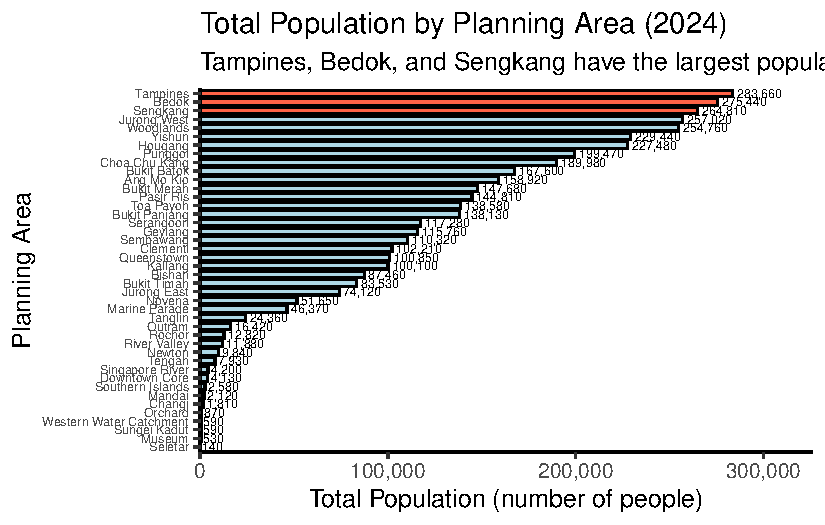
\includegraphics{Take-home_Ex01_files/figure-pdf/unnamed-chunk-22-1.pdf}




\end{document}
